\documentclass{article}
\usepackage{import}
\usepackage{float}
% \usepackage{emoji}
\usepackage{graphicx}
% \setemojifont{TwemojiMozilla}
% \usepackage{fontspec}

\title{Advanced Algorithms\\Homework 04}
\author{Felix Céard-Falkenberg\\7174020}

\usepackage{../homework} % See homework.sty %

\begin{document}

\section{Question 2}
\subsection{\textbf{Draw an example graph such that $k > 4$ and $n > 20$. Mark all the layers $V_1, \dots$ with a different color.}}

\begin{figure}[H]
  \centering
  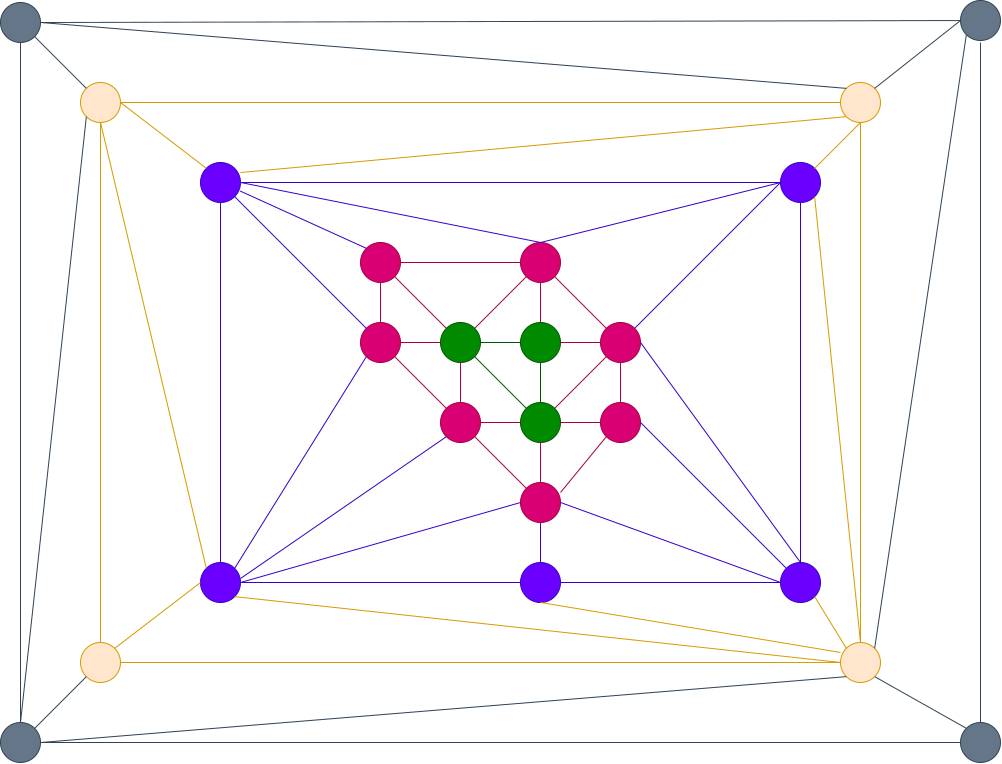
\includegraphics[width=\linewidth]{graph.pdf}
  \caption{THE {\fontfamily{pzc}\selectfont graph} \textgreater{}:3.}
  \label{fig:example-graph}
\end{figure}

\pagebreak
\subsection{\textbf{Show that there are paths of length at most $k$ from $V_1$ to $V_k$. If you take two of them together
you have a set of size $2k$ that separates the graph into at least two components. Assuming $k = O(\sqrt{n})$
we have a small separator of the graph. It is unclear if this separator is balanced. Describe a graph
together with two such paths that lead to an unbalanced separator.}}

We start by proving that there exists at least one path of length at most $k$ that connect $V_1$ to $V_k$. To this end, we will first prove a lemma to demonstrate that the graph in Figure~\ref{fig:graph-minimal} is the minimal graph for constructing $V_1$ and $V_2$.

\begin{figure}[tbp]
    \centering
    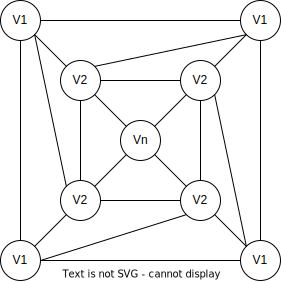
\includegraphics[width=0.5\linewidth]{minimal.pdf}
    \caption{The minimal graph for $V_1$ and $V_2$, where $V_n$ denotes the graph of the subsequent layers. Note that we assume that $V_n$ is a triangulation too; we exclude the empty set.}
    \label{fig:graph-minimal}
\end{figure}

\begin{lemma}
    The graph in Figure~\ref{fig:graph-minimal} contains the minimal number of nodes and edges for constructing $V_1$ and $V_2$, up to equivalence in their ordering.
    \label{lemma:minimal-graph}
\end{lemma}
\begin{proof}
    We can prove this lemma by using a proof by contradiction.

    \textbf{Edges.}
    Suppose that there exists an edge that can be removed, such that the graph still is a triangulation, and the sets $V_1$ and $V_2$ remain the same.
    In that case, the graph would not be minimal, as we could remove that edge and still have a triangulation.
    
    However, removing any edge between two nodes in $V_1$ (or two nodes in $V_2$) would result in at least one node of the subsequent layer being moved to a higher layer (e.g., a node $v\in V_2$ would be moved to the set $V_1$ if such an edge is removed). Hence, these edges are strictly necessary for the graph to be a triangulation.

    Furthermore, removing any edge between $V_1$ and $V_2$ in this graph would result a inner face between $V_1$ and $V_2$ to not be a triangle. This would violate the definition of a triangulation graph, and thus, these edges are strictly necessary too.

    We can reuse the same two arguments to show that the edges between $V_2$ and $V_n$ are strictly necessary too. Note that while we represent $V_n$ as a single node, in a real graph, $V_n$ is an entire graph, and thus the exact connection between $V_2$ and $V_n$ can differ based on the exact construction of $V_n$.
    Thus, all edges in this graph are stricly necessary for not violating the triangulation property, and therefore, the graph is the minimal graph for constructing $V_1$ and $V_2$ around a graph $V_n$.


    \textbf{Nodes.}
    By removing any node from this graph, we would move the outer face to a sub-layer, and therefore violate the constraint that the sets remain the same. Thus, all nodes in this graph are strictly necessary for not violating the triangulation property.

    Therefore, because every edge and node is strictly necessary for not violating the triangulation property, we can conclude that the graph in Figure~\ref{fig:graph-minimal} is the minimal graph for constructing $V_1$ and $V_2$ around a graph $V_n$.
\end{proof}

Before proving Theorem~\ref{thm:path-exists}, we will first introduce Lemma~\ref{lemma:add-nodes}, which will be used to prove the final theorem. 
% While we constrain the placement of the new nodes in Lemma~\ref{lemma:add-nodes
\begin{lemma}
    % Using the minimal graph for $V_1$ and $V_2$ from Figure~\ref{fig:graph-minimal}, 
    Given a triangulation graph, we can add an infinite number of nodes to each set $V_i$ while maintaining the triangulation property iff we constrain their placement to edges $(u, v)$, where $u, v \in V_i$.
    \label{lemma:add-nodes}
\end{lemma}
\begin{proof}
    Without loss of generality, we can assume that we have the minimal graph as shown in Figure~\ref{fig:graph-minimal}.
    To prove this lemma, we will prove both directions of the implication:

    $\Rightarrow$


    We prove this lemma using a proof by induction over the number of nodes added to a set $V_i$. 

    \textbf{Base case ($n=1$).}
    We can easily extend $V_i$ by one node by adding it on any edge $(u, v)$, where $u, v \in V_i$, as long as the position is not exactly $u$ or $v$. This can be easily shown as the edge $(u, v)$ is a straight line, and that the shape of the face is not affected by the addition of a single node on a straight line. Furthermore, as the new node is also incident to the same face as another node in $V_i$, the new node will be removed in $G_{i+1}$. Therefore, the new node does not affect the triangulation property of the graph.

    If however, we would place the new node on an edge $(u, w)$ where $u\in V_i$ and $w\notin V_i$ (either upper or lower layer), we would violate the triangulation property, as in the graph $G_i$, the new node would be "floating around", which would result in a non-triangular face, thus violating the triangulation property.

    \textbf{Induction step.}
    We can repeat the same argument, except that we now include the previously added nodes to the set $V_i$, as they are also incident to the same face as the new node. Therefore, the new node does not affect the triangulation property of the graph.

    $\Leftarrow$

    We repeat the same argument as before.
\end{proof}

% \begin{lemma}
%     In a triangulation graph, there always exists each node $v\in V_i$ is connected to at least one node $u\in V_{i+1}$.    
% \end{lemma}
% \begin{proof}
%     We show this by contradiction.
%     Let us assume, for the sake of contradiction, that for a node $v\in V_i$, there does not exist a node $u \in V_{i+1}$ with $(v, u) \in A$.
% \end{proof}

\begin{theorem}
    There exists at least one path of length at most $k$ from $V_1$ to $V_k$.
    \label{thm:path-exists}
\end{theorem}
\begin{proof}

    % We can easily show the existence of such a path by using a proof by contradiction.

    By combining Lemma~\ref{lemma:minimal-graph} and Lemma~\ref{lemma:add-nodes}, we know that it is possible to define the minimal structure of any triangulation graph for $V_i$ with $k > 2$ by recursively creating new graphs based on Figure~\ref{fig:graph-minimal}.
    
    Therefore, following from Lemma~\ref{lemma:add-nodes}, we know that there will always exist a direct connection from $V_i$ to $V_{i+1}$ for any $i \in \set{1, \dots, k-1}$, as adding nodes to these connecting edges violates the triangulation property. As each of these connecting edges between layers must lie on a direct path from $V_1$ to $V_k$, we know that there exists a path of length at most $k$ from $V_1$ to $V_k$.
    

    % Let us show the existence of such a path by induction over $k$.

    % \textbf{Base case ($k=2$).}
    % For $k=2$, we trivially have a direct connection from $V_1$ to $V_2$, as otherwise the graph can be separated into two distinct graphs, and we would have $V_1 = G_1$.

    % \textbf{Base case ($k=3$).}
    % The case $k=3$ is a bit more complicated. 

    % We use a proof by induction over $k$. Note that with $V$, we denote the set of vertices in the graph.
    % % Note that $k= 1$ is trivially true, hence we start with $k=2$.

    % \textbf{Base case ($k=2$).}
    % We have $k=2$. By removing the nodes contained in $V_1$, we obtain a new graph, which by definition is also a triangulation. Because $V_1$ and $V_2$ are directly connected by at least 6 edges,\!\footnote{No formal proof is given here, showing this is quite easy, but requires a bit of work that I do not want to do...} we know that there exists a path of length exactly 1 (and at most 2) from $V_1$ to $V_2$.
    % Therefore, a path of length at most $k$ exists connecting $V_1$ and $V_2$.

    % \textbf{Base case ($k=3$).}
    % For $k=3$, we have to use a finer argument. From the base case, we know that $V_1$ and $V_2$ are connected by a path of length 1 ($k-1$).
    % % Using the same argument as in the first base case, we know that there exists a path of length 1 between $V_2$ and $V_3$.
    % % However, while the path from $V_1$ to $V_2$ and from $V_2$ to $V_3$ may not be connected to the same node, we will always 
    % By following on path of length 1 from $V_1$ to $V_2$, we know that the node in which the path ends is connected to $V_3$ by at least one edge, as otherwise, the graph $V_2 \cup V_3$ (with the respective edges) would not be a triangulation.
    

    % \textbf{Induction step.}
    % % Let us now consider the case for $k+1$. Because we know that $V_1$ and $V_2$ are connected by a path of length at most $k$ 

\end{proof}


\end{document}
